\documentclass[12pt,a4paper]{article}
\usepackage[UTF8]{ctex}
\usepackage{amsmath}
\usepackage{graphicx}
\usepackage{booktabs}
\usepackage{geometry}
\usepackage{ulem}
\geometry{left=2.5cm,right=2.5cm,top=2.5cm,bottom=2.5cm}

\title{\Huge{\textbf{\uuline{实\ 验\ 报\ 告}}}}
\author{\uline{少年班学院} \quad 姓名: \uline{李大恕} \quad 学号: \uline{PB24000145} \quad 实验日期: \uline{2025--5--26}}
\date{\today}

\begin{document}

\maketitle

\section{实验题目}
	切变模量的测量

\section{实验目的}
    \begin{enumerate}
        \item 用扭摆来测量金属丝的切变模量；
        \item 学习尽量设法避免测量那些较难测准的物理量，从而提高实验精度的设计思想。
    \end{enumerate}

\section{实验原理}
    实验对象是一根上下均匀而细长的钢丝，从几何上说可以等效为一细长的圆柱体，其半径为$R$，长度为$L$。将其上端固定，而使其下端面发生扭转。扭转力矩使圆柱体各截面小体积元均发生切应变。

    在弹性限度内，且切应变$\gamma=R\frac{\mathrm d\varphi}{\mathrm dt}\ll 1$ 时，可将扭摆的转动类比于小振动，于是可以通过测量扭摆转动的周期，间接计算出钢丝的切变模量：
    \begin{equation}
        D = \frac{4\pi^2}{T_0^2}I_0
    \end{equation}
    \begin{equation}
        G = \frac{2DL}{\pi R^4}
    \end{equation}
    其中，$T_0$是扭摆不悬挂其他物体时的转动周期，$I_0$是扭摆对其悬挂点的转动惯量；但是因为扭摆的固定方式导致其转动惯量难以被测出，因此可将一个金属环对称地置于圆盘上。

    设这个金属环具有质量$m$，内半径$r_\text{内}$和外半径$r_\text{外}$，置于圆盘上后可得到转动周期$T_1$，利用比值法，可将上面的公式改写为：
    \begin{equation}
        D = \frac{2\pi^2 m (r_\text{内}^2 + r_\text{外}^2)}{T_1^2 - T_0^2}
    \end{equation}
    \begin{equation}
        G = \frac{4\pi L m (r_\text{内}^2 + r_\text{外}^2)}{R^4 (T_1^2 - T_0^2)}
    \end{equation}

    \begin{center}
        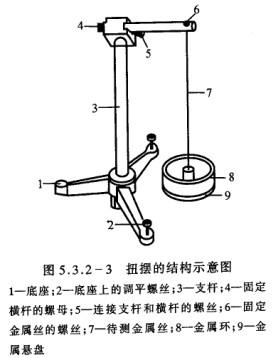
\includegraphics[width=0.4\textwidth]{实验装置示意图.jpg}\\
        \textbf{图1：扭摆实验装置示意图}
    \end{center}


\section{实验器材}
    \begin{itemize}
        \item 待测钢丝
        \item 扭摆及悬挂装置（其中待测钢丝下已经悬挂了圆盘）
        \item 已知质量的金属环
        \item 卷尺，游标卡尺，螺旋测微器，电子秒表
    \end{itemize}

\section{实验步骤}
    \begin{enumerate}
        \item 装置扭摆，使钢丝与作为扭摆的圆盘面垂直，圆环应能方便地置于圆盘上。
        \item 用螺旋测微器测钢丝直径，用游标卡尺测环的内外径，用米尺测钢丝的有效长度。
        \item 写出相对误差公式，据此估算应测多少个周期较合适。
        \item 计算钢丝的切变模量$G$和扭转模量$D$，分析误差。
    \end{enumerate}
        
\section{实验数据}
    \subsection{长度测量}
        测量钢丝长度、直径和圆环内外径的数据如下：
        \begin{center}
            \begin{tabular}{cccc}
                \toprule
                次数 & 1 & 2 & 3 \\
                \midrule
                $L/\mathrm{cm}$ & 40.30 & 40.29 & 40.30 \\
                \bottomrule
            \end{tabular} \\
            \textbf{表1：钢丝长度测量数据} \\
            [1em]
            \begin{tabular}{ccccccccccc}
                \toprule
                次数 & 1 & 2 & 3 & 4 & 5 & 6 & 7 & 8 & 9 & 10 \\
                \midrule
                $d/\mathrm{mm}$ & 0.799 & 0.802 & 0.797 & 0.797 & 0.798 & 0.802 & 0.800 & 0.797 & 0.801 & 0.796 \\
                \bottomrule
            \end{tabular} \\
            \textbf{表2：钢丝直径测量数据} \\
            [1em]
            \begin{tabular}{cccc}
                \toprule
                次数 & 1 & 2 & 3 \\
                \midrule
                $d_\text{内}/\mathrm{mm}$ & 8.360 & 8.380 & 8.378 \\
                $d_\text{外}/\mathrm{mm}$ & 10.390 & 10.392 & 10.390 \\
                \bottomrule
            \end{tabular} \\
            \textbf{表3：圆环内外径测量数据}
        \end{center}
    \subsection{质量测量}
        本实验中，实验室给定了金属圆环的质量$m = 577.7\,\mathrm{g}$。由于实验室测量金属圆环的方法、工具皆未知，测量次数未知，因此圆环的质量视为已知量处理，无需分析不确定度。
    \subsection{测量周期数的确定}
        根据相对误差公式，可以给出：
        \[
            \frac{\Delta G}{G} = \frac{\Delta L}{L} + \frac{\Delta m}{m} + 4\frac{\Delta R}{R} + \frac{2r_\text{内}\Delta r_\text{内}+2r_\text{外}\Delta r_\text{外}}{r_\text{内}^2+r_\text{外}^2}+\frac{2T_0\Delta T_0 + 2T_1\Delta T_1}{T_1^2 - T_0^2}
        \]
        
        其中，根据前面的数据进行估计，可以发现主要误差为$4\Delta R/R$项。而与周期有关的项不可直接求出，但是应当要求两者各自的误差小于主要误差的$1/5$。于是得到两个不等式：
        \[
            \frac{2T_1\Delta T_1}{T_1^2 - T_0^2} < \frac{1}{5}\frac{4\Delta R}{R}
        \]
        \[
            \frac{2T_0\Delta T_0}{T_1^2 - T_0^2} < \frac{1}{5}\frac{4\Delta R}{R}
        \]
        对扭摆周期进行估测，并考虑到人使用秒表计时时的误差为 $\Delta T = 0.2\,\mathrm{s}$，可解出大约需要40个周期。
        
        所以接下来本实验中每次测量均使扭摆摆动40个完整周期。
    \subsection{周期测量}
        由于实验室的扭摆装置不便于直接测量转动惯量，因此采用比值法，测量周期。先测量不悬挂金属环时的转动周期$T_0$，然后将金属环放在圆盘上，测量转动周期$T_1$。每次测量均记录40个完整周期的时间，数据如下：
        \begin{center}
            \begin{tabular}{ccccc}
                \toprule
                次数 & 1 & 2 & 3 & 4 \\
                \midrule
                $40T_0/\mathrm{s}$ & 79.21 & 79.17 & 79.17 & 79.20 \\
                $40T_1/\mathrm{s}$ & 128.57 & 128.52 & 128.56 & 128.55 \\
                \bottomrule
            \end{tabular} \\
            \textbf{表4：扭摆周期测量数据}
        \end{center}

\section{数据处理与误差分析}
    钢丝直径$d$的平均值
    \[
        \overline{d}=\frac{1}{n}\sum_{i=1}^{n}d_i=0.7989\,\mathrm{mm}
    \]

    钢丝直径$d$的标准差
    \[
        \begin{aligned}
            \sigma_{d}&=\sqrt{\frac{1}{n-1}\sum_{i=1}^n\left(d_i-\overline{d}\right)^2}\\
            &=0.0022336\,\mathrm{mm}
        \end{aligned}
    \]

    钢丝直径$d$的B类不确定度
    \[
        \Delta_{B,d}=\sqrt{\Delta_\text{仪}^2+\Delta_\text{估}^2}=\sqrt{0.01^2+0.005^2}\,\mathrm{mm}=0.01118\,\mathrm{mm}
    \]

    钢丝直径$d$的展伸不确定度
    \[
        \begin{aligned}
            U_{d,P}&=\sqrt{\left(t_P\frac{\sigma_{d}}{\sqrt{n}}\right)^2+\left(k_P\frac{\Delta_{B,d}}{C}\right)^2}\\
            &=\sqrt{\left(2.26\times\frac{0.0022336}{\sqrt{10}}\right)^2+\left(1.96\times\frac{0.01118}{3}\right)^2}\,\mathrm{mm}\\
            &=7.4769 \times 10^{-3}\,\mathrm{mm},P=0.95
        \end{aligned}
    \]

    环内直径$d_\text{内}$的平均值
    \[
        \overline{d_\text{内}}=\frac{1}{n}\sum_{i=1}^{n}{d_\text{内}}_i=83.727\,\mathrm{mm}
    \]

    环内直径$d_\text{内}$的标准差
    \[
        \begin{aligned}
            \sigma_{d_\text{内}}&=\sqrt{\frac{1}{n-1}\sum_{i=1}^n\left({d_\text{内}}_i-\overline{d_\text{内}}\right)^2}\\
            &=0.11015\,\mathrm{mm}
        \end{aligned}
    \]

    环内直径$d_\text{内}$的B类不确定度
    \[
        \Delta_{B,d_\text{内}}=0.02\,\mathrm{mm}
    \]

    环内直径$d_\text{内}$的展伸不确定度
    \[
        \begin{aligned}
        U_{d_\text{内},P}&=\sqrt{\left(t_P\frac{\sigma_{d_\text{内}}}{\sqrt{n}}\right)^2+\left(k_P\frac{\Delta_{B,d_\text{内}}}{C}\right)^2}\\
        &=\sqrt{\left(4.3\times\frac{0.11015}{\sqrt{3}}\right)^2+\left(1.96\times\frac{0.02}{\sqrt{3}}\right)^2}\,\mathrm{mm}\\
        &=0.2744\,\mathrm{mm},P=0.95
        \end{aligned}
    \]

    环外直径$d_\text{外}$的平均值
    \[
        \overline{d_\text{外}}=\frac{1}{n}\sum_{i=1}^{n}{d_\text{外}}_i=103.91\,\mathrm{mm}
    \]

    环外直径$d_\text{外}$的标准差
    \[
        \begin{aligned}
            \sigma_{d_\text{外}}&=\sqrt{\frac{1}{n-1}\sum_{i=1}^n\left({d_\text{外}}_i-\overline{d_\text{外}}\right)^2}\\
            &=0.011547\,\mathrm{mm}
        \end{aligned}
    \]

    环外直径$d_\text{外}$的B类不确定度
    \[
        \Delta_{B,d_\text{外}}=0.02\,\mathrm{mm}
    \]

    环外直径$d_\text{外}$的展伸不确定度
    \[
        \begin{aligned}
            U_{d_\text{外},P}&=\sqrt{\left(t_P\frac{\sigma_{d_\text{外}}}{\sqrt{n}}\right)^2+\left(k_P\frac{\Delta_{B,d_\text{外}}}{C}\right)^2}\\
            &=\sqrt{\left(4.3\times\frac{0.011547}{\sqrt{3}}\right)^2+\left(1.96\times\frac{0.02}{\sqrt{3}}\right)^2}\,\mathrm{mm}\\
            &=0.036524\,\mathrm{mm},P=0.95
        \end{aligned}
    \]

    钢丝长度$L$的平均值
    \[
        \overline{L}=\frac{1}{n}\sum_{i=1}^{n}L_i=40.297\,\mathrm{cm}
    \]

    钢丝长度L的标准差
    \[
        \begin{aligned}
            \sigma_{L}&=\sqrt{\frac{1}{n-1}\sum_{i=1}^n\left(L_i-\overline{L}\right)^2}\\
            &=0.0057735\,\mathrm{cm}
        \end{aligned}
    \]

    钢丝长度$L$的B类不确定度
    \[
        \Delta_{B,L}=\sqrt{\Delta_\text{仪}^2+\Delta_\text{估}^2}=\sqrt{0.1^2+0.05^2}\,\mathrm{cm}=0.1118\,\mathrm{cm}
    \]

    钢丝长度$L$的展伸不确定度
    \[
        \begin{aligned}
            U_{L,P}&=\sqrt{\left(t_P\frac{\sigma_{L}}{\sqrt{n}}\right)^2+\left(k_P\frac{\Delta_{B,L}}{C}\right)^2}\\
            &=\sqrt{\left(4.3\times\frac{0.0057735}{\sqrt{3}}\right)^2+\left(1.96\times\frac{0.1118}{3}\right)^2}\,\mathrm{cm}\\
            &=0.074438\,\mathrm{cm},P=0.95
        \end{aligned}
    \]

    周期$T_0$的平均值
    \[
        \overline{T_0}=\frac{1}{n}\sum_{i=1}^{n}{T_0}_i=1.9797\,\mathrm{s}
    \]

    周期$T_0$的标准差
    \[
        \begin{aligned}
        \sigma_{T_0}&=\sqrt{\frac{1}{n-1}\sum_{i=1}^n\left({T_0}_i-\overline{T_0}\right)^2}\\
        &=0.00051539\,\mathrm{s}
        \end{aligned}
    \]

    周期$T_0$的B类不确定度
    \[
        \Delta_{B,T_0}=\sqrt{\Delta_\text{仪}^2+\Delta_\text{估}^2}=\sqrt{0.0005^2+0.01^2}\,\mathrm{s}=0.010012\,\mathrm{s}
    \]

    周期$T_0$的展伸不确定度
    \[
        \begin{aligned}
            U_{T_0,P}&=\sqrt{\left(t_P\frac{\sigma_{T_0}}{\sqrt{n}}\right)^2+\left(k_P\frac{\Delta_{B,T_0}}{C}\right)^2}\\
            &=\sqrt{\left(3.18\times\frac{0.00051539}{\sqrt{4}}\right)^2+\left(1.96\times\frac{0.010012}{3}\right)^2}\,\mathrm{s}\\
            &=6.5926 \times 10^{-3}\,\mathrm{s},P=0.95
        \end{aligned}
    \]

    周期$T_1$的平均值
    \[
        \overline{T_1}=\frac{1}{n}\sum_{i=1}^{n}{T_1}_i=3.2138\,\mathrm{s}
    \]
    
    周期$T_1$的标准差
    \[
        \begin{aligned}
            \sigma_{T_1}&=\sqrt{\frac{1}{n-1}\sum_{i=1}^n\left({T_1}_i-\overline{T_1}\right)^2}\\
            &=0.00054006\,\mathrm{s}
        \end{aligned}
    \]

    周期$T_1$的B类不确定度
    \[
        \Delta_{B,T_1}=\sqrt{\Delta_\text{仪}^2+\Delta_\text{估}^2}=\sqrt{0.0005^2+0.01^2}\,\mathrm{s}=0.010012\,\mathrm{s}
    \]

    周期$T_1$的展伸不确定度
    \[
        \begin{aligned}
            U_{T_1,P}&=\sqrt{\left(t_P\frac{\sigma_{T_1}}{\sqrt{n}}\right)^2+\left(k_P\frac{\Delta_{B,T_1}}{C}\right)^2}\\
            &=\sqrt{\left(3.18\times\frac{0.00054006}{\sqrt{4}}\right)^2+\left(1.96\times\frac{0.010012}{3}\right)^2}\,\mathrm{s}\\
            &=6.5976 \times 10^{-3}\,\mathrm{s},P=0.95
        \end{aligned}
    \]

    扭转模量
    \[
        D=\frac{\pi^{2} m \left(d_{1}^{2} + d_{2}^{2}\right)}{- 2 T_{0}^{2} + 2 T_{1}^{2}}=7.9207 \times 10^{-3}\,\mathrm{N·m}
    \]

    扭转模量$D$的延伸不确定度
    \[
        \begin{aligned}
            U_{D,P}&=\sqrt{\left(\frac{\partial D}{\partial d_\text{内}}U_{d_\text{内},P}\right)^2+\left(\frac{\partial D}{\partial d_\text{外}}U_{d_\text{外},P}\right)^2+\left(\frac{\partial D}{\partial T_1}U_{T_1,P}\right)^2+\left(\frac{\partial D}{\partial T_0}U_{T_0,P}\right)^2}\\
            &=6.4934 \times 10^{-5}\,\mathrm{N·m},P=0.95
        \end{aligned}
    \]

    扭转模量最终结果
    \[
        D=\left(0.00792 \pm 0.00007\right)\,\mathrm{kg·m^2/s^2}
    \]

    切变模量
    \[
        G=\frac{16 \pi L m \left(d_{1}^{2} + d_{2}^{2}\right)}{d^{4} \left(- T_{0}^{2} + T_{1}^{2}\right)}=7.9811 \times 10^{10}\,\mathrm{Pa}
    \]

    切变模量$G$的延伸不确定度
    \[
        U_{G,P}=3.0638 \times 10^{9}\,\mathrm{Pa},P=0.95
    \]

    切变模量最终结果
    \[
        G=\left(8.0 \pm 0.3\right) \times 10^{10}\,\mathrm{Pa}
    \]

    相对不确定度$\eta \approx 3.8\% < 5\%$，满足实验要求。

\section{思考题}
    \begin{enumerate}
        \item \textbf{本实验是否满足$\gamma\ll 1$的要求？} \\
            以$\varphi=180^\circ$ 为例，此时最大切应变 $\gamma_{\max} = R\varphi/L \approx 0.003 \ll 1$，所以小幅摆动的条件是成立的。
        \item \textbf{为提高测量精度，本实验在设计上作了哪些安排？在具体测量时又要注意什么？} \\
            设计上，设法避免测量较难测准的物理量。难以测量扭转角度，于是使用扭摆法，通过测量扭摆运动周期计算切变模量。难以直接测量转动惯量，转化为通过过比较加减金属环前后的转动惯量变化导致的周期变化，计算切变模量。

            操作上，实验前先估算，求得需要测量的周期数，避免测量周期数过少导致的误差过大；测量前，调整扭摆装置，使钢丝与扭摆的圆盘面垂直。扭转扭摆时，确保钢丝尽量垂直、扭摆绕固定轴转动。
    \end{enumerate}

\appendix
    \section{老师签字的原始数据}
        \begin{center}
            
\includegraphics[width=0.8\textwidth]{原始数据.jpg}
        \end{center}

\end{document}
